\documentclass[journal,12pt,twocolumn]{IEEEtran}
\usepackage{setspace}
\usepackage{gensymb}
\singlespacing
\usepackage[cmex10]{amsmath}

\usepackage{amsthm}
\usepackage{hyperref}
\hypersetup{
    colorlinks=true,
    linkcolor=blue,
    filecolor=magenta,      
    urlcolor=cyan,
}

\urlstyle{same}
\usepackage{mathrsfs}
\usepackage{txfonts}
\usepackage{stfloats}
\usepackage{bm}
\usepackage{cite}
\usepackage{cases}
\usepackage{subfig}

\usepackage{longtable}
\usepackage{multirow}

\usepackage{enumitem}
\usepackage{mathtools}
\usepackage{steinmetz}
\usepackage{tikz}
\usepackage{circuitikz}
\usepackage{verbatim}
\usepackage{tfrupee}
\usepackage[breaklinks=true]{hyperref}
\usepackage{graphicx}
\usepackage{tkz-euclide}
\usetikzlibrary{shapes,backgrounds}
\usepackage{verbatim}
\usetikzlibrary{calc,math}
\usepackage{listings}
    \usepackage{color}                                            %%
    \usepackage{array}                                            %%
    \usepackage{longtable}                                        %%
    \usepackage{calc}                                             %%
    \usepackage{multirow}                                         %%
    \usepackage{hhline}                                           %%
    \usepackage{ifthen}                                           %%
    \usepackage{lscape}     
\usepackage{multicol}
\usepackage{chngcntr}
\usepackage{mdframed}
\DeclareMathOperator*{\Res}{Res}

\renewcommand\thesection{\arabic{section}}
\renewcommand\thesubsection{\thesection.\arabic{subsection}}
\renewcommand\thesubsubsection{\thesubsection.\arabic{subsubsection}}

\renewcommand\thesectiondis{\arabic{section}}
\renewcommand\thesubsectiondis{\thesectiondis.\arabic{subsection}}
\renewcommand\thesubsubsectiondis{\thesubsectiondis.\arabic{subsubsection}}


\hyphenation{op-tical net-works semi-conduc-tor}
\def\inputGnumericTable{}                                 %%

\lstset{
%language=C,
frame=single, 
breaklines=true,
columns=fullflexible
}

\usepackage{chngcntr}
\counterwithin{figure}{section}

\title{AI5002}
\author{TUHIN DUTTA}
\date{January 2021}

\begin{document}
\newtheorem{theorem}{Theorem}[section]
\newtheorem{problem}{Problem}
\newtheorem{proposition}{Proposition}[section]
\newtheorem{lemma}{Lemma}[section]
\newtheorem{corollary}[theorem]{Corollary}
\newtheorem{example}{Example}[section]
\newtheorem{definition}[problem]{Definition}

\newcommand{\BEQA}{\begin{eqnarray}}
\newcommand{\EEQA}{\end{eqnarray}}
\newcommand{\define}{\stackrel{\triangle}{=}}
\bibliographystyle{IEEEtran}
\raggedbottom
\setlength{\parindent}{0pt}
\providecommand{\mbf}{\mathbf}
\providecommand{\pr}[1]{\ensuremath{\Pr\left(#1\right)}}
\providecommand{\qfunc}[1]{\ensuremath{Q\left(#1\right)}}
\providecommand{\sbrak}[1]{\ensuremath{{}\left[#1\right]}}
\providecommand{\lsbrak}[1]{\ensuremath{{}\left[#1\right.}}
\providecommand{\rsbrak}[1]{\ensuremath{{}\left.#1\right]}}
\providecommand{\brak}[1]{\ensuremath{\left(#1\right)}}
\providecommand{\lbrak}[1]{\ensuremath{\left(#1\right.}}
\providecommand{\rbrak}[1]{\ensuremath{\left.#1\right)}}
\providecommand{\cbrak}[1]{\ensuremath{\left\{#1\right\}}}
\providecommand{\lcbrak}[1]{\ensuremath{\left\{#1\right.}}
\providecommand{\rcbrak}[1]{\ensuremath{\left.#1\right\}}}
\theoremstyle{remark}
\newtheorem{rem}{Remark}
\newcommand{\sgn}{\mathop{\mathrm{sgn}}}

\providecommand{\res}[1]{\Res\displaylimits_{#1}} 

%\providecommand{\norm}[1]{\lVert#1\rVert}
\providecommand{\mtx}[1]{\mathbf{#1}}
\providecommand{\fourier}{\overset{\mathcal{F}}{ \rightleftharpoons}}
%\providecommand{\hilbert}{\overset{\mathcal{H}}{ \rightleftharpoons}}
\providecommand{\system}{\overset{\mathcal{H}}{ \longleftrightarrow}}
	%\newcommand{\solution}[2]{\textbf{Solution:}{#1}}
\newcommand{\solution}{\noindent \textbf{Solution: }}
\newcommand{\cosec}{\,\text{cosec}\,}
\providecommand{\dec}[2]{\ensuremath{\overset{#1}{\underset{#2}{\gtrless}}}}
\newcommand{\myvec}[1]{\ensuremath{\begin{pmatrix}#1\end{pmatrix}}}
\newcommand{\mydet}[1]{\ensuremath{\begin{vmatrix}#1\end{vmatrix}}}
\numberwithin{equation}{subsection}
\makeatletter
\@addtoreset{figure}{problem}
\makeatother
\let\StandardTheFigure\thefigure
\let\vec\mathbf
\renewcommand{\thefigure}{\theproblem}
\def\putbox#1#2#3{\makebox[0in][l]{\makebox[#1][l]{}\raisebox{\baselineskip}[0in][0in]{\raisebox{#2}[0in][0in]{#3}}}}
     \def\rightbox#1{\makebox[0in][r]{#1}}
     \def\centbox#1{\makebox[0in]{#1}}
     \def\topbox#1{\raisebox{-\baselineskip}[0in][0in]{#1}}
     \def\midbox#1{\raisebox{-0.5\baselineskip}[0in][0in]{#1}}
\vspace{3cm}
\title{AI5002 - Challenge Problem 9}
\author{Tuhin Dutta\\ ai21mtech02002}
\maketitle
\newpage
\bigskip
\renewcommand{\thefigure}{\theenumi}
\renewcommand{\thetable}{\theenumi}
\begin{mdframed}
Download code and LaTeX from below hyperlinks\\
1. \href{https://github.com/Tauhait/AI5002/tree/main/Challenge-Problem/9/LaTeX}{LaTeX}
\end{mdframed}
\subsection*{\boldsymbol{Problem\ \textbf{IES\_ISS\_2015\_stat1\_Q3c}}}
Two points are chosen on a line of unit length. Find the probability that each of the 3 line segments will have length greater than $\dfrac{1}{4}$?
\subsection*{\boldsymbol{Solution}}
\begin{figure}[h!]
    
\includegraphics[width=\columnwidth]{Challenge-Problem/9/Figure/LineSeq2.png}
    \centering \caption*{Fig 1: Line Segment}
\end{figure}
We can choose two points randomly say $P_1$, and $P_2$. Let the length of the first segment from 0 to $P_1$ be $X$, length of the second segment from $P_1$ to $P_2$ be $Y$, and length of the third segment from $P_2$ to $1$ be $1-X-Y$.

We want the length of each of the segments to be
\begin{align}\tag{1}
    X & > \dfrac{1}{4}
\end{align}
\begin{align}\tag{2}
    Y & > \dfrac{1}{4}
\end{align}
\begin{align}\tag{3}
    1-X-Y & > \dfrac{1}{4}\ or\ X + Y < \dfrac{3}{4}
\end{align}
Let us plot these three inequalities (1), (2), and (3) in the X-Y plane as shown in Fig 2.
\begin{figure}[h!]
    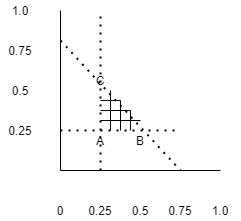
\includegraphics[width=\columnwidth]{Challenge-Problem/9/Figure/LineSeq1.png}
    \centering \caption*{Fig 2: Favourable and Total Area}
\end{figure}
From figure 2 we see that all three inequalities are satisfied in the highlighted area marked by A, B and C.\\
$\therefore$
\begin{align}\tag{4}
    \begin{split}
        Favourable\ Area &= \dfrac{1}{2}\cdot\text{BASE}\cdot\text{HEIGHT}\\
                        &= \dfrac{1}{2}\cdot(B-A)\cdot(C-A)\\
                        &= \dfrac{1}{2}\cdot(\dfrac{1}{2}-\dfrac{1}{4})\cdot(\dfrac{1}{2}-\dfrac{1}{4})\\
                        &= \dfrac{1}{32}
    \end{split}
\end{align}
Now to calculate the sample space or total area we have is the triangle with points at (0, 0), (0,1), and (1, 0).\\
$\therefore$
\begin{align}\tag{5}
    \begin{split}
        Total\ Area &= \dfrac{1}{2}\cdot\text{BASE}\cdot\text{HEIGHT}\\
                        &= \dfrac{1}{2}\cdot(1-0)\cdot(1-0)\\
                        &= \dfrac{1}{2}
    \end{split}
\end{align}
$\therefore$
\begin{align}\tag{6}
    \begin{split}
        &\pr{X > \dfrac{1}{4}\ and\ Y > \dfrac{1}{4} and\ X + Y < \dfrac{3}{4}}\\
    &= \dfrac{\text{Favourable\ Area}}{\text{Total\  Area}}\\
    &= \dfrac{1/32}{1/2}\\
    &= \dfrac{1}{16}
\end{split}
\end{align}
\end{document}
